\documentclass[colorlinks=true,pdfstartview=FitV,linkcolor=blue,
            citecolor=red,urlcolor=magenta]{ligodoc}

\usepackage{graphicx}
\usepackage{amssymb}
\usepackage{amsmath}
\usepackage{longtable}
\usepackage{rotating}
\usepackage[usenames,dvipsnames]{color}
\usepackage{fancyhdr}
\usepackage{subfigure}
\usepackage{hyperref}
% \usepackage{minted}
\usepackage{appendix}
\usepackage{tikz}
\usetikzlibrary{shapes,arrows,fit}
\ligodccnumber{T}{19}{00287}{}{v1}% \ligodistribution{AIC, ISC}


\title{Data Clustering Techniques for the Correlation of Environmental Noise to Signals in LIGO Detectors}

\author{Jacob Bernhardt, Anamaria Effler, Rana Adhikari}

\begin{document}

\section{Introduction}
The LIGO project uses laser interferometry to measure gravitational waves (GWs).
LIGO interferometers transduce their relative arm length differences caused by GWs to a signal composed of optical power, known as DARM.

Due to the amplitude scales of GWs, The LIGO detectors have to operate at a very high sensitivity; the spectral density of a measurable length difference is as low as $2\times 10^{-20}~\mathrm{m}/\sqrt{\mathrm{Hz}}$ at 100 Hz.
The design of earthbound LIGO is thus heavily focused on the filtering and isolation of environmental noise.

To help identify and characterize environment-based noise, the LIGO detector has a Physical Environment Monitoring (PEM) system, a diverse array of environmental sensors positioned all over the facility\cite{aepaper}.
This is used for a multitude of purposes, including the data quality report (DQR), which aims to veto segments of time by finding correlations between PEM and DARM through statistical inference and sometimes also supervised learning.
Supplementing coincidence analysis between the two detectors, DQR prevents GW-like noise transients from being falsely categorized as events.

Both detector livetime and detection range can be increased by figuring out how to decouple environmental noise from DARM.
Directly coupling noise, found by basic coherence, has been already addressed, but the complexity of the detector causes many noise sources to up- or down-convert.
These require some more careful statistical correlation to identify, and are sometimes not well understood.
\begin{figure}
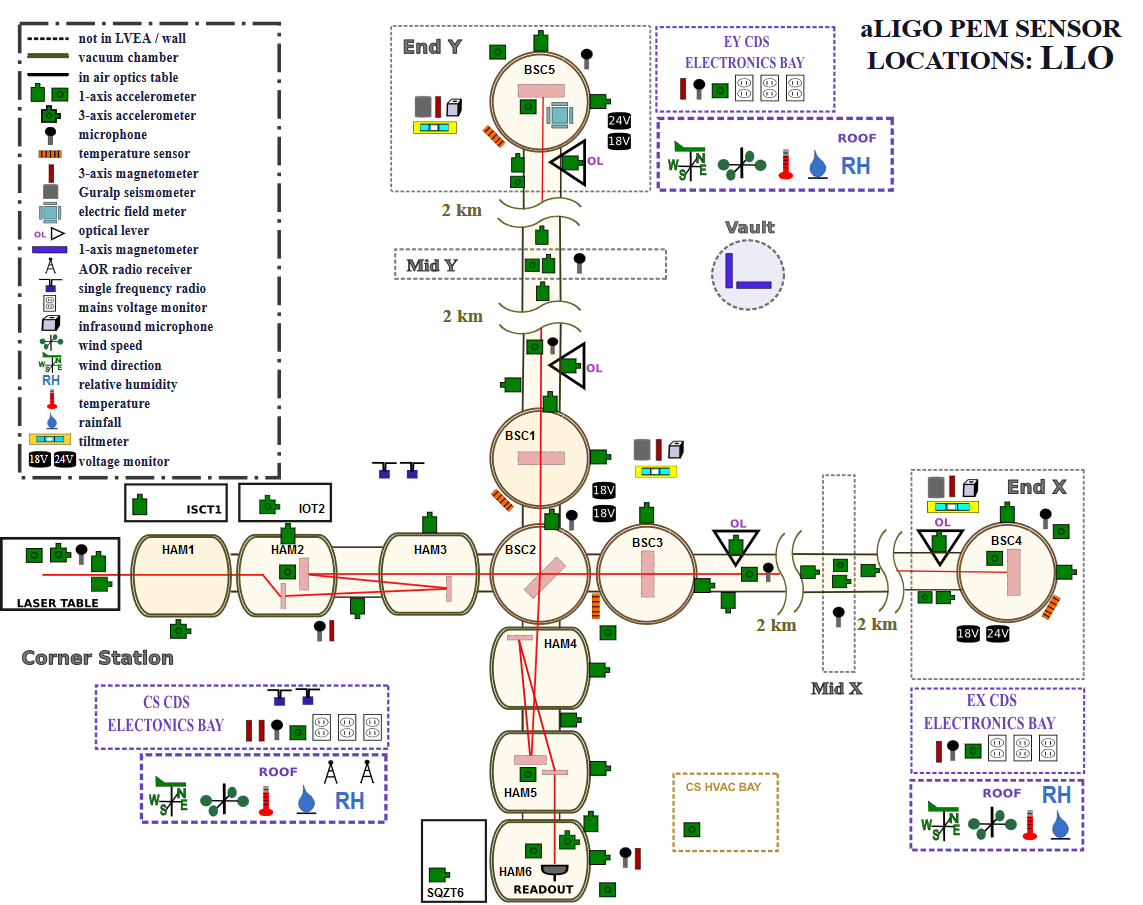
\includegraphics[width=\textwidth]{assets/llopem.png}
\caption{Schematic PEM map at the LIGO Livingston Observatory (L1). Shaded areas are in vacuum.}
\end{figure}
\begin{figure}
  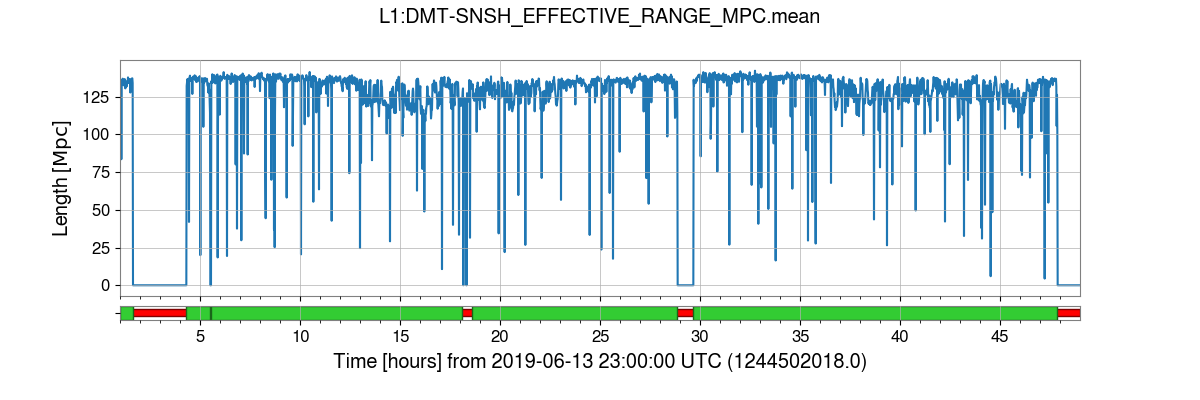
\includegraphics[width=\textwidth]{assets/L1:DMT-SNSH_EFFECTIVE_RANGE_MPC.png}
  \caption{Detector range at L1 seems to consistently reduce during the day ($\sim$6am-5pm CST), thought to result from anthropic activity. This can be as much as 10 Mpc for NS-NS mergers.}
\end{figure}

Separating noise sources out of a signal can be considered a clustering problem in a space covering different frequency bands in which noise appears.
A previous LIGO SURF student has evaluated several data clustering algorithms with respect to their ability to properly sort out frequency elements of seismometer signals caused by specific earthquake events\cite{roxana}.
Both the $k$-means algorithm, which aims to make clusters with low standard deviation, and the DBSCAN algorithm, which minimizes overall inter-point distance in clusters, were evaluated using multiple methods, including the Calinsky-Harabaz  index and direct comparison to earthquake times via time labeling of points, ultimately showing poor earthquake identification.
A long short-term memory (LSTM) recurrent neural network (RNN) seemed to work much better, but due to small input sample size, this solution may have been be plagued by over-fitting.
Thus, it is imperative that a more robust frequency clustering mechanism be designed for the PEM system.

\section{Objectives}
\begin{enumerate}
\item
  Find an algorithm or clustering approach which correctly identifies known noise events.
\item
  Use the results of (1) to create a clustering approach to discover previously unknown noise correlations and/or sources.
\end{enumerate}

\section{Approach}

A program was written to take the spectral power of any PEM channel, in the form of band-limited RMS (BLRMS) by summing in-band bins of a power spectrogram, with inspiration from \cite{vajente}. By clustering spectral bands of PEM channels, frequency conversions could be accounted for.

A Python script was written to perform the an initial clustering approach, explained in Section~\ref{sec:kmeans}, with a variety of tunable parameters. It was validated on a regime with known noise states, the seismometers, satisfying the first objective. No other clustering approach was extensively investigated (Appendix~\ref{app:algo}).

Unknown noise states in accelerometers and microphones were clustered using this approach, to meet the second objective. (Section~\ref{sec:unknown}).

To glean the correlations between frequencies in clustered channels, a script was created to visually present the power in frequencies in channels by cluster. This is explained in Section~\ref{ssec:eval}.

\section{$k$-Means Clustering with Histories}\label{sec:kmeans}
The $k$-means algorithm was used to cluster the two hours of minute-trend data preceding each point in time.
The coordinates of a clustered point were as follows:
\begin{equation}
  \begin{array}{c}
    \{s_0(t_0),s_0(t_{-1}),s_0(t_{-2}),\cdots,s_0(t_{-n}),\\
    s_1(t_0),s_1(t_{-1}),s_1(t_{-2}),\cdots,s_1(t_{-n}),\\
    s_2(t_0),s_2(t_{-1}),s_2(t_{-2}),\cdots,s_2(t_{-n}),\\
    \cdots,\\
    s_m(t_0),s_m(t_{-1}),s_m(t_{-2}),\cdots,s_m(t_{-n})\}
  \end{array}
\end{equation}
with $s_j(t)$ the value of a clustered channel $j$ at time $t$ in its own units, e.g. a seismometer velocity at time $t$.
Each dimension could be thought of as ``value of specific channel a specific number of minutes ago'', allowing trends over time to be matched together in a phase-agnostic way.
This yields a cluster space of dimensionality (\# of channels) $\times$ (\# of minutes of history).

Notably, the clustering endeavored by \cite{roxana} lacked this history feature, using a clustering space of dimensionality (\# of channels) $\times$ (1).
Instead of just finding times when the channels are similar in value, the history clustering is sensitive to the shape of clustered features.

\begin{figure}[h]
  \tikzstyle{block} = [rectangle, draw, text width=6em, text centered, rounded corners, minimum height=4em]
  \begin{tikzpicture}[node distance = 9em, auto]
    \node [block] (dl) {get minute-trend data from NDS};
    \node [block, right of=dl] (input) {create input matrix};
    \node [block, right of=input] (compute) {compute $k$-means clusters};
    \node [block, right of=compute] (save) {save labels};
    \draw [->] (dl) -- (input);
    \draw [->] (input) -- (compute);
    \draw [->] (compute) -- (save);
  \end{tikzpicture}
  \caption{Clustering script flowchart. The clustering algorithm creates a time series of cluster numbers, a label for each minute of clustered time.}
\end{figure}

\subsection{Sanity Checking with Seismometers}
For a total clustering duration of 30 days, using the seismometers attached to ETMY, ETMX, and ITMY, in minute-trend half-order-of-magnitude BLRMS bands from 30 mHz to 30 Hz, the following known noise events were easily identified using a ``2-hour history'' $k$-means method:
\begin{itemize}
\item earthquakes ($0.01\to0.1$ Hz)
\item microseism ($0.1\to1$ Hz)
\item anthropogenic noise ($1\to10$ Hz)
\end{itemize}

A microseism is a faint seismic tremor caused by natural processes, such as waves of pressure in the ocean, which happens over the course of hours. All human activity creates so-called ``anthropogenic noise'', and cars, trains, logging, and even footsteps can couple to DARM. The noise floor at anthropogenic-noise-dominated frequencies noticeably rises during the day and lowers during the night. Loud human-originated events, such as trains passing, stand out over even the daytime noise floor.

Some differentiation between subcategories of events in the same frequency band but of different timescales (e.g. earthquakes vs. wind; train vs. noise from cars) was lacking.

\begin{figure}[h]\hspace{-2ex}
  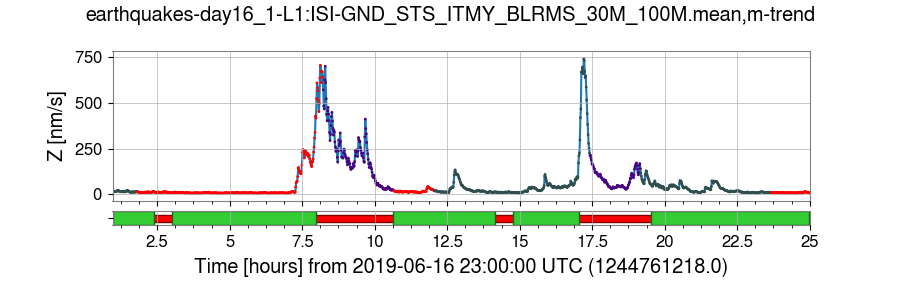
\includegraphics[width=0.7\textwidth]{assets/final/earthquakes-day16_1-L1:ISI-GND_STS_ITMY_BLRMS_30M_100Mmean,m-trend.png}
  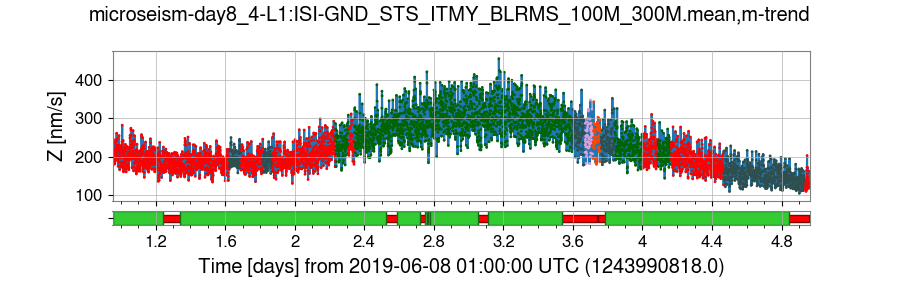
\includegraphics[width=0.7\textwidth]{assets/final/microseism-day8_4-L1:ISI-GND_STS_ITMY_BLRMS_100M_300Mmean,m-trend.png}
  \caption{Seismic BLRMS near clustered earthquakes (above, purple, 30 mHz $\to$ 0.1 Hz) and microseism (below, green, 0.1 Hz $\to$ 0.3 Hz)}
\end{figure}

The length of the history was initially thought to have an effect on the timescales of identifiable events; experimentation (namely, trying 30-minute and 6-hour histories on the same data) showed that this is not really true.

The next idea was that there were too many different types of features in too large a space for events with a small number of points, like the trains, to be separated out.
The test was re-run with only anthropogenic seismic BLRMS bands at the end stations, which yielded very clear distinction between the anthropogenic noise types (See Figure~\ref{fig:trains}).

\begin{figure}
  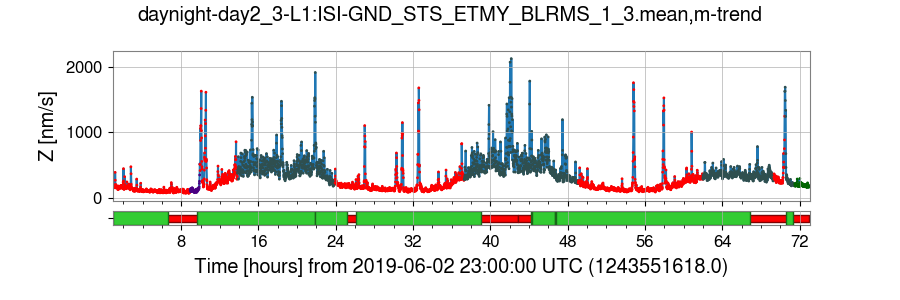
\includegraphics[width=0.7\textwidth]{assets/final/daynight-day2_3-L1:ISI-GND_STS_ETMY_BLRMS_1_3mean,m-trend.png}
  
  \raggedleft{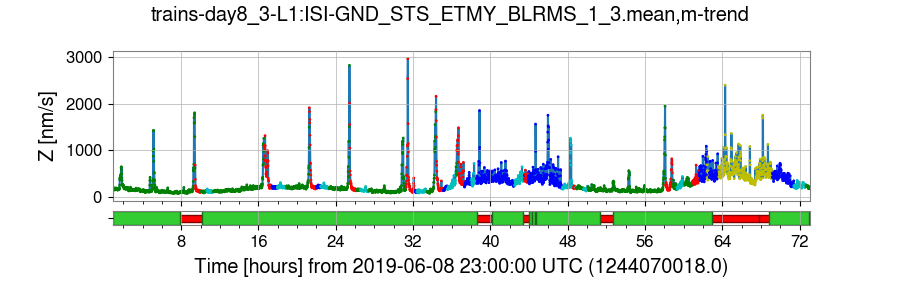
\includegraphics[width=0.7\textwidth]{assets/final/trains-day8_3-L1:ISI-GND_STS_ETMY_BLRMS_1_3mean,m-trend.png}}
  \caption{Seismic BLRMS from 1 Hz $\to$ 3 Hz. Using all bands, the $k$-means approach clustered all anthropogenic features together (above, gray). Limiting the clustering space allowed short events like trains (red, below) to be separated out from day/night variation (blue, below).}\label{fig:trains}
\end{figure}

\section{Clustering of Unknown Noise States}\label{sec:unknown}
Now that the clustering scheme was verified using known states of noise, it could be used to find new relationships between PEM channels and DARM noise.

\subsection{Microphones}\label{ssec:mic}

A ``2-hour history'' $k$-means method was used to cluster 30 days of data from microphones in the LVEA, XVEA and YVEA in BLRMS bands shown in Table~\ref{tab:blrms}.
\begin{table}\centering
  \begin{tabular}{l|l|l}
    DARM & MIC & ACC \\
    \hline \hline
    \begin{tabular}[t]{@{}l@{}}
      10-13 \\
      18-22 \\
      22-27 \\
      27-29 \\
      29-40 \\
      40-54 \\
      54-65 \\
      65-76 \\
      75-115 \\
      115-190 \\
      190-210 \\
      210-290 \\
      290-480 \\
      526-590 \\
      590-650 \\
      650-885 \\
      885-970 \\
      1110-1430
    \end{tabular} &
    \begin{tabular}[t]{@{}l@{}}
      10-28 \\
      28-32 (HVAC) \\
      32-50 \\
      50-70 \\
      70-100 \\
      100-200
    \end{tabular} &
    \begin{tabular}[t]{@{}l@{}}
      1-4 \\
      4-10 \\
      10-28 \\
      28-32 \\
      32-48 \\
      48-60 \\
      60-80 \\
      80-118 \\
      118-122 \\
      122-200
    \end{tabular}\\
    \hline
  \end{tabular}
  \caption{Selected clustering BLRMS bands [Hz].}\label{tab:blrms}
\end{table}
Two interesting ``noisy'' states were identified: a relatively quiet, multi-hour cluster, and a quick, loud cluster.
Tables of the median percent increase of amplitude in certain BLRMS bands with respect to the largest cluster in the run (representative of the noise floor) are shown in Table~\ref{tab:mic}, and their spectra in Figure~\ref{fig:mic}.

\begin{table}\hspace{2em}
  \begin{tabular}{l|llr}
    Hz & 10-28 & 28-32 & 32-50 \\ \hline
    LVEA & 109\% & 95\% & 176\% \\
    XVEA & 87\% &   &  89\% \\
    YVEA & 131\% & 83\% & 165\%
  \end{tabular}\hfill
  \begin{tabular}{l|lr}
    Hz & 32-50 & 50-70 \\ \hline
    LVEA & 1112\% & 890\% \\
    PLUSX & 1183\% & 1034\% \\
    PLUSY & 1100\%
  \end{tabular}\hspace{2em}
  \caption{Percent increase tables (see Section~\ref{ssec:eval}) for clustered acoustic long, quiet (left) and short, loud (right) states.}\label{tab:mic}
\end{table}

The clustering was repeated with observing segments of \texttt{L1:GDS-CALIB\_STRAIN} included.
This produced approximately the same clusters as before, likely because segmenting of DARM added weight to the MIC channels.
The cluster corresponding to the same longer, quieter ``noisy'' state occured during locked times, so its effect on DARM was examined.
As shown in Table~\ref{tab:micdarm}, there was a slight average increase in DARM during the cluster.
This difference can also be seen in the representative spectrum (see Section~\ref{ssec:eval}) of the cluster (Figure~\ref{fig:mic}).
Nevertheless, the noise state does not impact DARM significantly enough to be useful for sensitivity improvements.

\begin{table}\centering
  \begin{tabular}{l|llr}
    Hz & 22-27 & 27-29 & 29-40 \\ \hline
    \texttt{GDS-CALIB\_STRAIN} & 1\% & 3\% & 1\%
  \end{tabular}
  \caption{Percent increase table (see Section~\ref{ssec:eval}) for the DARM component of the longer, quieter acoustic cluster.}\label{tab:micdarm}
\end{table}

\begin{figure}
  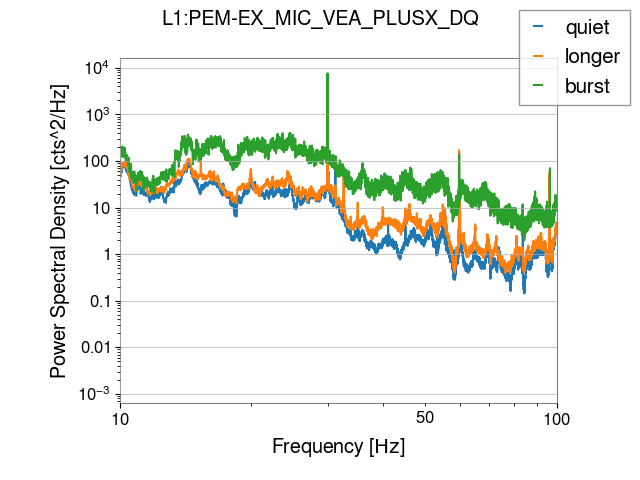
\includegraphics[width=0.5\textwidth]{assets/final/L1_PEM-EX_MIC_VEA_PLUSX_DQ.png}
  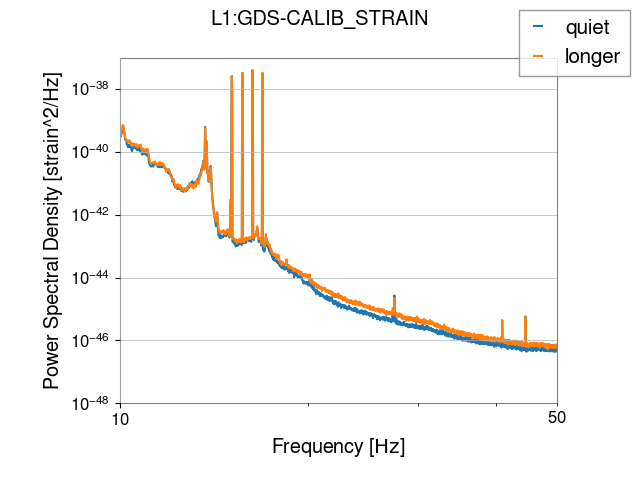
\includegraphics[width=0.5\textwidth]{assets/final/L1_GDS-CALIB_STRAIN-mic.png}
  \caption{Representative spectra (see Section~\ref{ssec:eval}) for acoustic states mentioned in Section~\ref{ssec:mic}. ``Quiet'' refers to the background ``everything else'' cluster. The orange cluster seems to affect DARM very little.}\label{fig:mic}
\end{figure}


\subsection{Accelerometers}
The ``2-hour history'' $k$-means method was used to cluster 30 days of data from various accelerometers from all VEAs in BLRMS bands shown in Table~\ref{tab:blrms}.
This was done in two groups, one with mostly BSC accelerometers and one focusing on beamtube motion.
The primary feature that clustered out in both runs was a 60 Hz motion at the mid stations increasing over half of a day.
After making representative spectra (Figure~\ref{fig:acc}), it was concluded that this noise was due to the HVAC system turning on during the warmer period of the day.
Motor load causes electrical signals to downconvert slightly as they couple into mechanical movement, so a peak at 58 Hz is characteristic of a fan.
The fan movement did not couple into DARM.

\begin{table}
  \begin{tabular}{l|llr}
    Hz    &       48-60 & 60-80 & 80-118 \\ \hline
    MY VEA BTUBE & 256\% & 259\% & 123\% \\
    EY BSC5 Z  &  108\% \\
  \end{tabular}\hfill
  \begin{tabular}{l|lr}
    Hz         &      48-60 & 54-65 \\ \hline
    MY 2100Y BTUBE &  618\%   & \\
    \texttt{GDS-CALIB\_STRAIN}  &&     38\%
  \end{tabular}
  \caption{Percent increase tables (see Section~\ref{ssec:eval}) for the 58 Hz accelerometer cluster. There appears to be a correlation to DARM, but looking at the cluster spectrum (Figure~\ref{fig:acc}) reveals this to be due to random fluctuations in the 60 Hz line.}\label{tab:acc}
\end{table}


\begin{figure}
  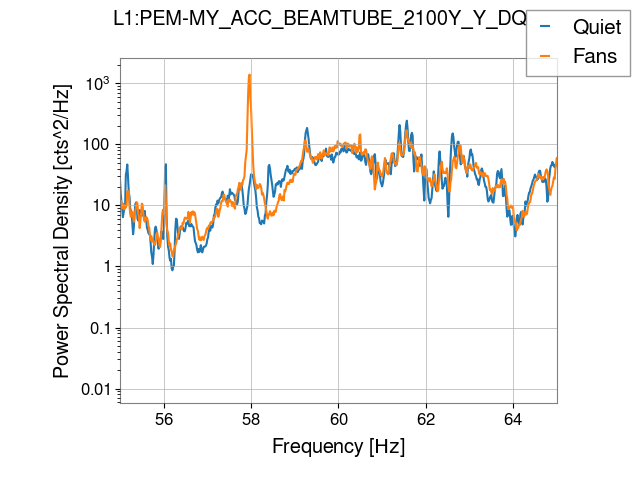
\includegraphics[width=0.5\textwidth]{assets/final/L1_PEM-MY_ACC_BEAMTUBE_2100Y_Y_DQ.png}
  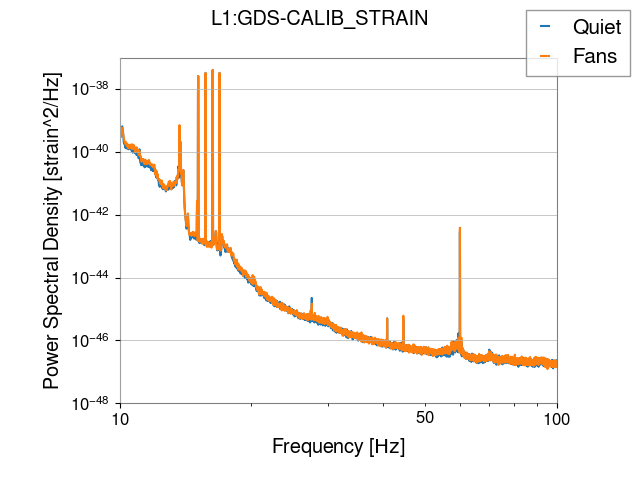
\includegraphics[width=0.5\textwidth]{assets/final/L1_GDS-CALIB_STRAIN-acc.png}
  \caption{Representative spectra (see Section~\ref{ssec:eval}) for the accelerometer noise state due to the fans at the mid-stations turning on. This manifests itself as a peak at 58 Hz. There is no coupling to DARM.}\label{fig:acc}
\end{figure}


\section{Developed Code Tools}
Many times, scientists are inclined to quickly do their simple calculations imperatively.
But time and RAM are not infinite, and with a high-output experiment like LIGO the usual kinds of scripts and operations do not suffice.
\subsection{Streaming}
One data-wrangling strategy is by programming with a ``streaming'' rather than ``batch'' mentality.
Many of the gravitational wave search pipelines have the ability to keep up with new LIGO data as it is collected, doing their batch-style work in short chunks, or strides, as the data comes along.
This keeps the execution footprint of the program managable, while allowing it to operate on an unending amount of data.

The Python package \texttt{GWpy}, used in this project, is the modern equivalent to LIGO's Algorithms Library, a set of common routines designed for LIGO data.
Strangely, appending to HDF5 savefiles, a streaming requisite, is not possible in \texttt{GWpy} without some lower-level calculations using the \texttt{libhdf5} wrapper directly and likely unintented \texttt{GWpy} keyword-argument usage.

Two helper functions, \texttt{write\_to\_disk} and \texttt{data\_exists}, were defined in \texttt{util.py} for the purpose of apppending a time series to an existing file and quickly checking the length of saved data without reading it.

A Python module was written to implement the ``streaming'' idea for any given batch operation.
One such task is the computation of BLRMS for channels that don't provide it in DMT frames.
The BLRMS-generating function is an implementation of a general \texttt{PostProcessor} interface, a \texttt{python3.7} dataclass which is fed INI options upon construction (see Figure~\ref{fig:pp}).
\begin{figure}[h]
  \tikzstyle{block} = [rectangle, draw, text width=6em, text centered, rounded corners, minimum height=4em]
  \tikzstyle{section} =[rectangle, draw, inner sep=1.125em, dashed]
  \begin{tikzpicture}[node distance = 9em, auto]
    \node [block] (dl) {get data from NDS or savefiles};
    \node [block, below of=dl] (strides) {compute strides};
    \node [block, right of=strides] (next) {get next stride};
    \node [block, below of=next] (stride) {extract stride};
    \node [block, right of=stride] (compute) {compute spectogram};
    \node [block, right of=compute] (add) {add power within requested bands};
    \node [block, right of=add] (save) {stitch stride into .hdf5 file};
    \node [block, below of=add] (shape) {read .hdf5 dataset shape};
    \node [block, below of=save] (offset) {compute offset};
    \node [section, label=below:BLRMS \texttt{PostProcessor}, fit=(add) (compute)] (blrms) {};
    \node [block, above of=blrms, node distance = 18em, dashed] (load) {load INI section};
    \draw [->] (dl) -- (strides);
    \draw [->] (strides) -- (next);
    \draw [->] (next) -- (stride);
    \draw [->] (stride) -- (compute);
    \draw [->] (compute) -- (add);
    \draw [->] (add) -- (save);
    \draw [->] (stride) |- (shape);
    \draw [->] (shape) -- (offset);
    \draw [->] (offset) -- (save);
    \draw [->] (save) |- (next);
    \draw [->, dashed] (load) -- (blrms);
    \draw [->, dashed] (load) -- (dl);
  \end{tikzpicture}
  \caption{States of the ``streaming post-processor'' script.}\label{fig:pp}
\end{figure}

Any data processing function which maps an input channel to an output channel and has tons of configuration parameters can take advantage of the module by implementing the \texttt{PostProcessor} interface.
Indeed, converting saved channels to minute-trend and caching NDS downloads in the same format were easy last-minute tasks with this generic structure in place.

\subsection{Evaluation of Clusters}\label{ssec:eval}
The clustering script itself was fairly straightforward, using the high abstraction provided by \texttt{scikit-learn}.
However, some thought was put into extracting meaning from the clusters.

A script was created to make power spectra for the clustered data representative of each cluster.
This is done by taking the median of the 1-minute power spectra for minutes clustered together.
An example of this is shown in Figure~\ref{fig:reps}.
\begin{figure}[h]
  \tikzstyle{block} = [rectangle, draw, text width=6em, text centered, rounded corners, minimum height=4em]
  \tikzstyle{section} =[rectangle, draw, inner sep=1.125em, rounded corners, ->]
  \begin{tikzpicture}[node distance = 9em, auto]
    \node [block] (labels) {read labels};
    \node [block, left of=labels] (filter) {locate base cluster};
    \node [block, left of=filter] (segments) {locate non-base cluster segments};
    \node [block, left of=segments] (dl) {download full-rate minutes in segments};
    \node [block, below of=segments] (psd) {take  psd for each minute in the cluster};
    \node [block, right of=psd] (median) {plot median};
    \node [section, label=above:for each cluster, fit=(psd) (median)] (cluster) {};
    \draw [->] (labels) -- (filter);
    \draw [->] (filter) -- (segments);
    \draw [->] (segments) -- (dl);
    \draw [->] (dl) |- (cluster);
    \draw [->] (psd) -- (median);
  \end{tikzpicture}
  \caption{Roughly the states of the ``representative spectra'' script. The most complicated overlooked detail in this figure is the caching of downloads. The stream writing functions used in the BLRMS-generation script have been moved and are now included from a more general location.}
\end{figure}

Taking the spectra of the clusters allows new states to be categorized without re-clustering, and a way to easily identify frequency conversion that is happening during coupling.

\begin{figure}
  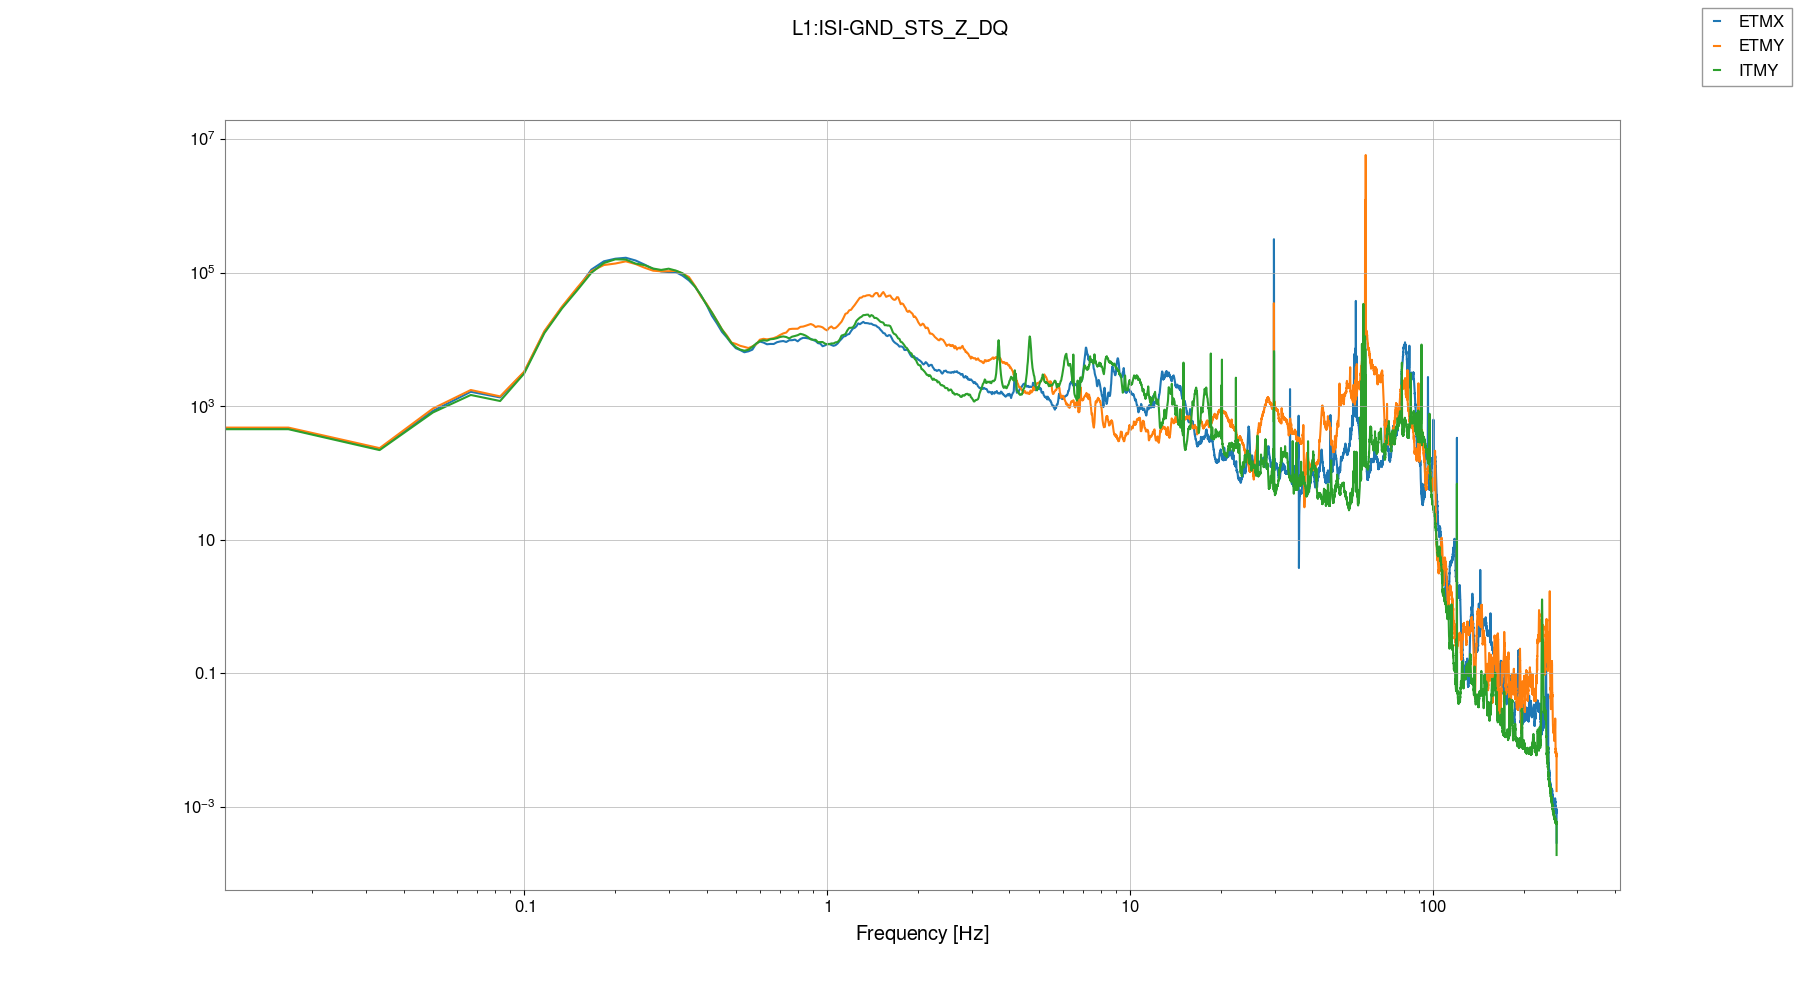
\includegraphics[width=\textwidth]{assets/report2/0-L1:ISI-GND_STS_Z_DQ.png}
  \caption{The representative spectrum of a cluster corresponding to train-dominated times. Notice that between 1 and 10 Hz, the seismic motion at ETMY (orange) is greater than at the other VEAs by a factor of about 10.}\label{fig:reps}
\end{figure}

In addition, the script can produce a table that shows which frequency bands are significant in each channel during clustered times.
This is done by taking the median percent increase in value of the minute-trend BLRMS of the each channel in each band.
The values in Tables~\ref{tab:mic},~\ref{tab:micdarm}, and~\ref{tab:acc} were all produced by this script, but handpicked from the rest of the output for clarity.


\appendix
\appendixpage
\section{Resampling}
Downloading and saving full-rate data takes an exorbitant amount of disk space, especially when only a portion of the frequency content is going to be used.
This calls for a decimation procedure to be applied to raw downloads before they are saved.

At CIT, Rana mentioned that the default low-pass filtering options in scipy's resampling function produce significant aliasing noise ($>1$\%) when downsampling by a large factor.
According to a test\footnote{see \url{https://git.ligo.org/NoiseCancellation/GWcleaning/issues/2}} done by Eric Quintero, this issue can be remedied without sacrificing runtime by using (1) a number of FIR taps proportional to the downsampling factor, rather than the default fixed value, and (2) a non-default window (\texttt{blackmanharris}).

% FIXME: figure of window comparison

For a full-rate time series \texttt{raw: gwpy.timeseries.TimeSeries}, the fastest and best procedure for resampling to \texttt{rate: int [Hz]} would be something like
% \begin{minted}[style=colorful]{python}
\begin{verbatim}
raw.resample(n=20*raw.sample_rate.value/rate, window='blackmanharris', rate=rate)
\end{verbatim}
% \end{minted}

\section{Evaluation of Non-$k$-means Clustering Algorithms}\label{app:algo}
A test\footnote{\url{https://scikit-learn.org/stable/auto_examples/cluster/plot_cluster_comparison.html}} which swaps out the $k$-means algorithm for others implemented in \texttt{sklearn} was executed to probe the geometry of the clusters.
From a first glance, the Spectral Clustering and Gaussian Mixture algorithms seemed to generalize better than $k$-means over different feature timescales.
However, algorithm upgrades are helpful only after tools for full cluster analysis are in place, and due to time limitations they were not revisited.

\begin{thebibliography}{2}
\bibitem{aepaper} A. Effler, R. M. S. Schofield, V. V. Frolov, G. Gonz{\'{a}}lez, K. Kawabe, J. R. Smith, J. Birch, and R. McCarthy, Classical and Quantum Gravity \textbf{32}, 035017 (2015).
\bibitem{roxana} LIGO Document T1700198-v1
\bibitem{vajente} aLIGO LLO Logbook entry 45374 by Gabriele Vajente
\end{thebibliography}



\end{document}
